\chapter{到達性を考慮したホスト選択手法}

前述のように,従来手法ではリストに基づくホスト選出を行っていた.待ち時間内に新ホストからのパケットを受信できなかったノードが,メインのネットワークに合流できず,ネットワーク分断が生じる可能性があった.本研究では,より安定的な転送制御を実現するために,到達性を考慮したホスト選択手法を提案する.提案するホスト選択手法を用いた同時送信フラッディングのフローチャートを図\ref{fig:ctf_te}に示す.
ここで到達性を考慮したホスト選択手法とは,媒介中心性と次数中心性によるホスト選択である.これらの算出にはネットワーク全体の隣接行列が既知であることが前提であり,トポロジー情報を保持しない従来の同時送信フラッディングにおいては適用できない.しかし,本研究では,事前のメッセージ交換等により隣接情報を取得しているものとする.そのため,センサノードの位置や距離が既知であり,ノードの位置変更もないという前提でシミュレーションを行う.また,先行研究~\cite{LoRa}の実験によって290\si{\meter}$\times$195\si{\meter}の範囲内ではノードの粗密に関わらず同時送信フラッディングの有効性が確認されているため,ノードの配置範囲を250\si{\meter}四方とした.

\begin{figure}[H]
  \centering
  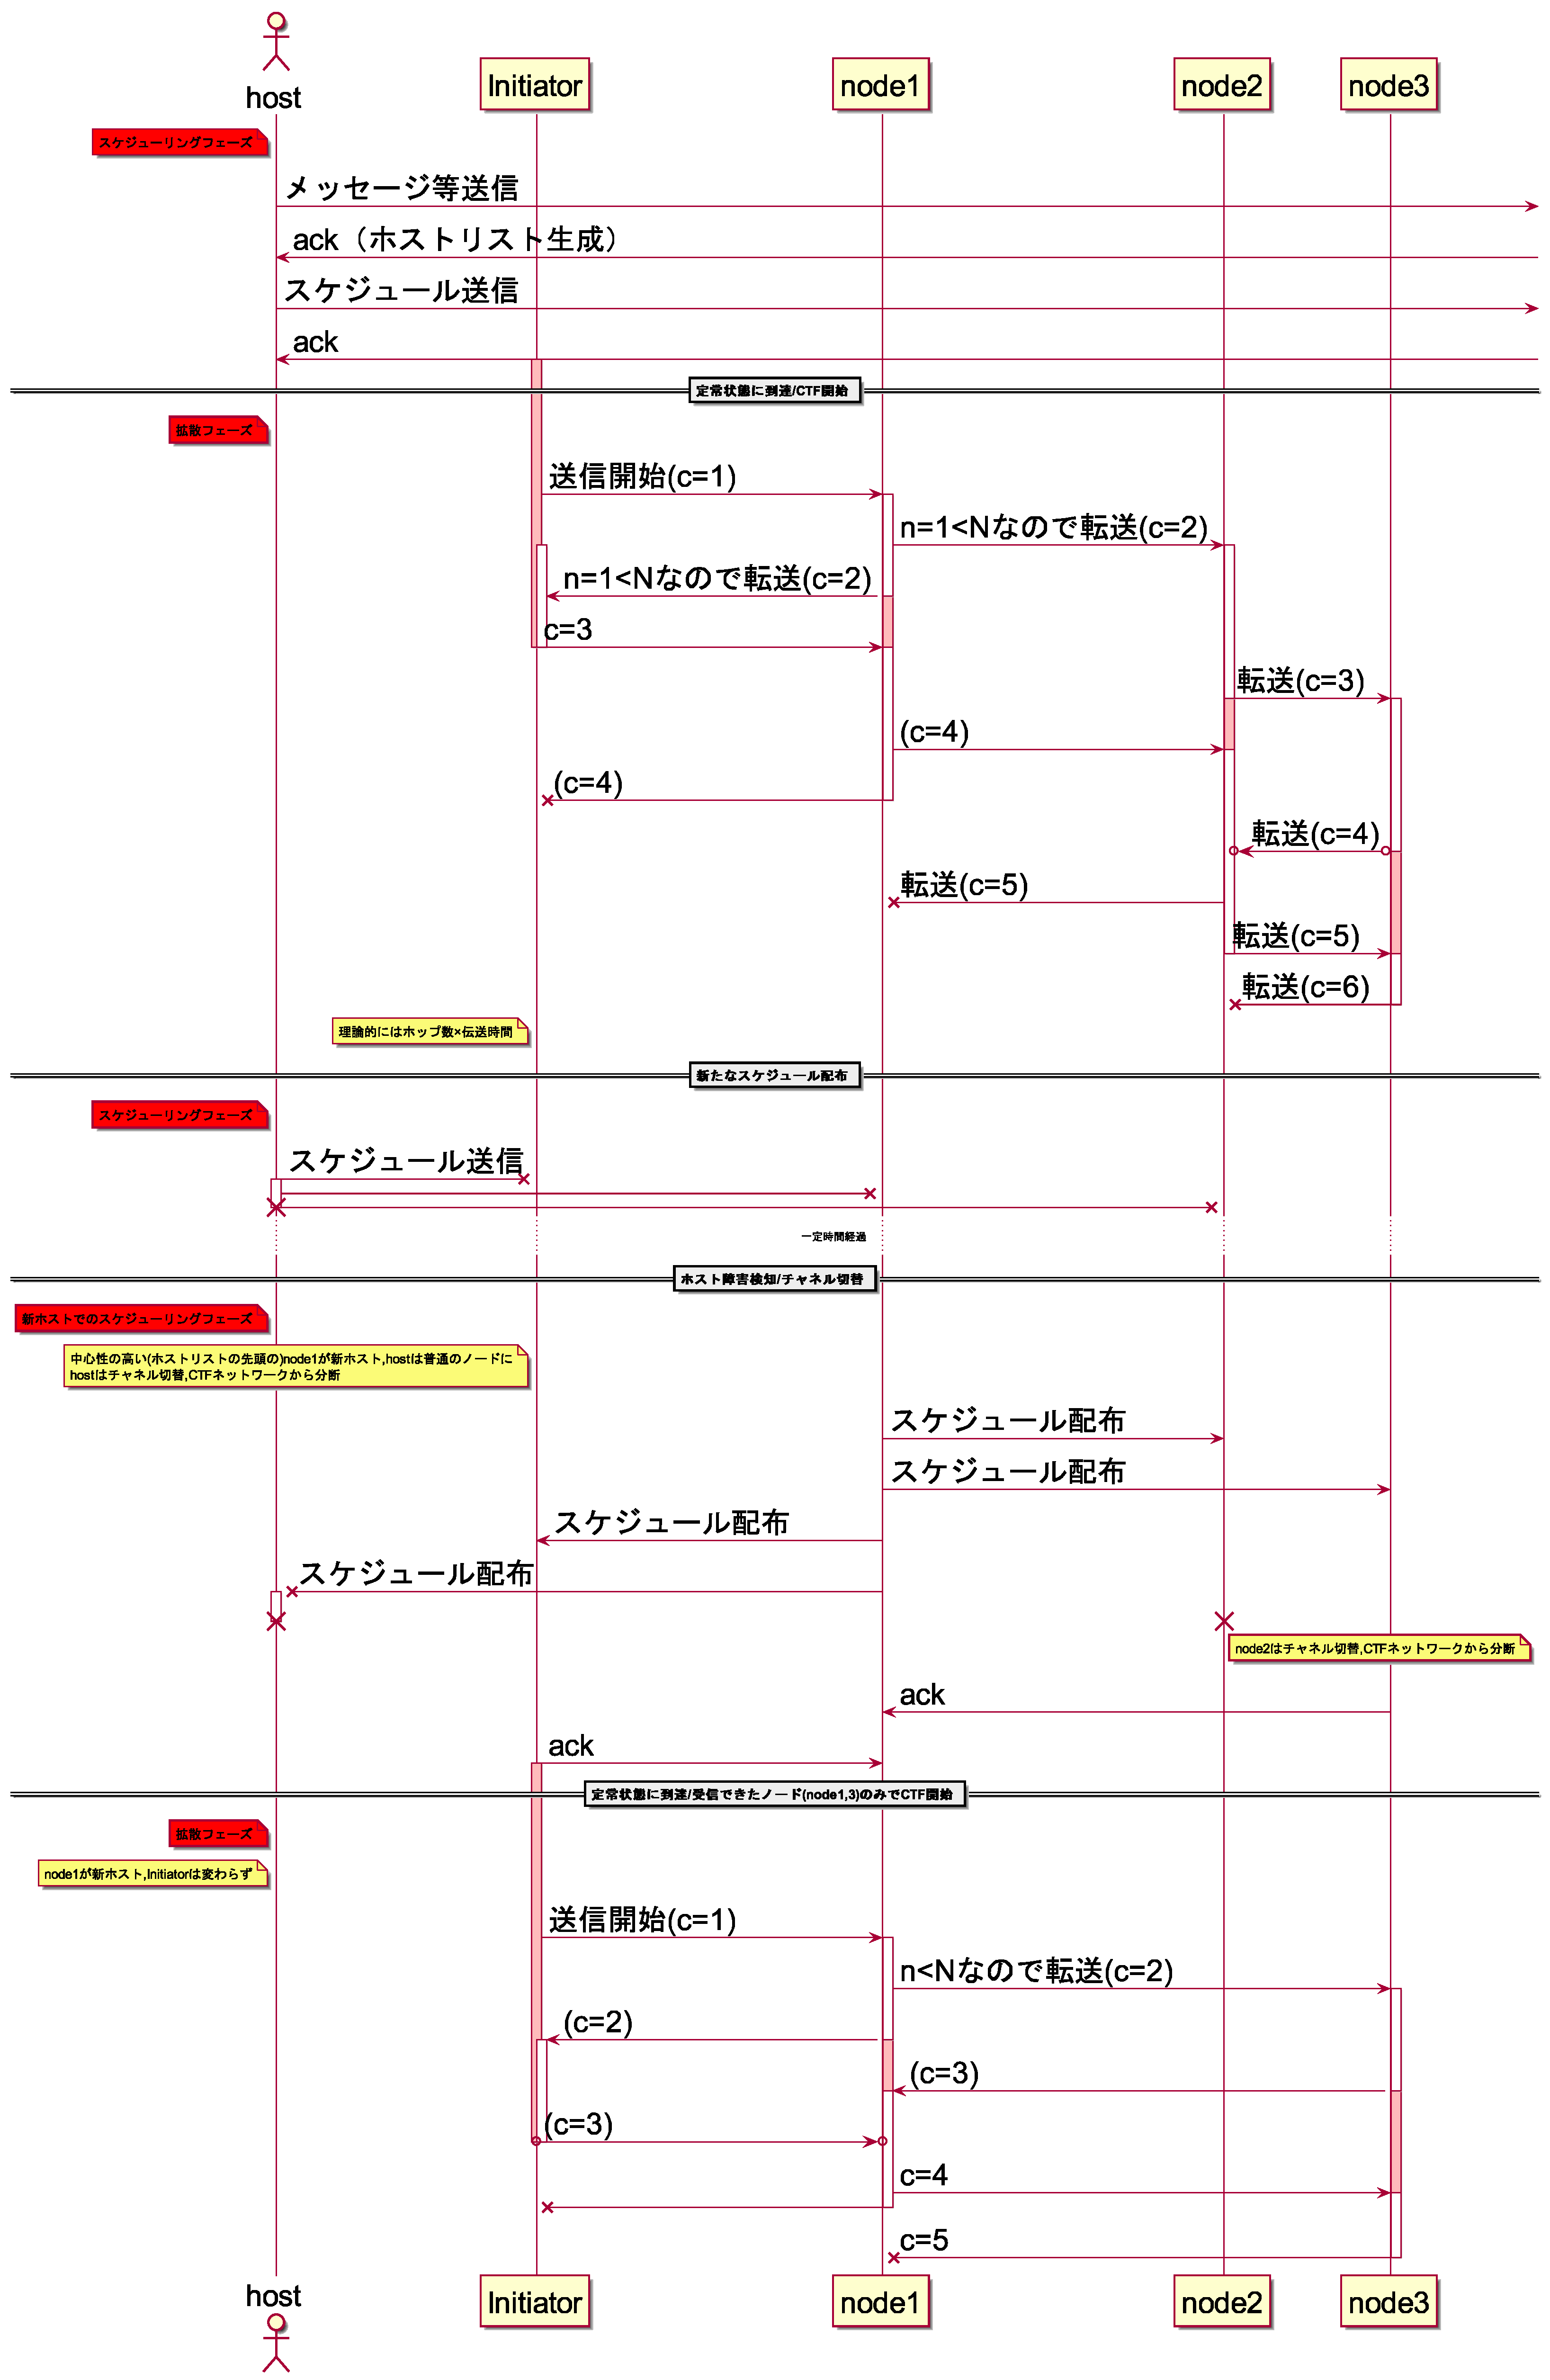
\includegraphics[width=1\textwidth]{figures/sequence_teian.eps}
  \caption{同時送信フラッディングの提案フローチャート}
  \label{fig:ctf_te}
\end{figure}

\section{ネットワークとグラフ}
\cite{network}によると,頂点と辺の具体的な関係性をネットワークという.本研究においてセンサを頂点,センサ同士の通信を辺と見なせばこれらの関係性もネットワークであると言える.またこれらは,頂点集合をV,辺の集合をEとすると,グラフG=(V,E)で定義できる.また,頂点間の繋がりが双方向なグラフを無向グラフという.本研究では無向グラフを考える.
また,どの頂点と頂点が繋がっているかを0と1で表す行列を隣接行列という.本研究で無向グラフを考えるため,隣接行列Aは対称であり,a[i,j]=a[j,i]となる.なおノードが自身から自身へ通信を行うことはあり得ないため,隣接行列の対角成分は0とする.図\ref{fig:adj}に示す.

\begin{figure}[H]
  \centering
  \includegraphics[width=0.8\textwidth]{figures/9.pdf}
  \caption{ノードと隣接行列}
  \label{fig:adj}
\end{figure}

\section{ホスト選択指標}
ホスト適性は,ノードの中心性に基づき評価を行う.
一般に,中心性とはネットワーク上におけるノードの重要性を評価するための指標であり,主な中心性の指標として媒介中心性や次数中心性が知られている.
\subsection*{媒介中心性}
媒介中心性は,そのノードが最短経路にどれくらい含まれるかを示す値である.この値が高いノードは,そのノードが失われたときにネットワーク全体に重大な影響を及ぼすことを意味する.本研究では,ネットワーク分断を避けるため,媒介中心性の高いノードをホストノードとしたい.そのためホスト選択指標として媒介中心性を使用する.あるグラフの隣接行列G=($g_{jk}$)を考えるとき,媒介中心性は以下の式\ref{eq_bet}で表せる.なお,$C_{b}(i)$は頂点iの媒介中心性,nはグラフ内の頂点数である.$g_{jk}$は頂点jと頂点kの間の全最短経路数で,$g_{jk}(i)$はその中で頂点iを通る数である.
\begin{equation}
\label{eq_bet}
C_{b}(i)=\sum_{i\neq j\neq l} \frac{g_{jk}(i)}{g_{jk}}
\end{equation}
\subsection*{次数中心性}
次数は,頂点に接続している辺の数である.次数中心性とはより多くの頂点と繋がっている頂点を高く評価する指標である.
本研究では,できるだけ多くのノードと通信可能なノードをホストノードとしたい.そのためホスト選択に次数中心性を使用する.あるグラフの隣接行列G=($g_{ij}$)を考えるとき,次数中心性は以下の式\ref{eq_deg}で表せる.なお,$C_{d}(i)$は頂点iの次数中心性,nはグラフ内の頂点数である.
\begin{equation}
\label{eq_deg}
C_{d}(i)=\sum_{j=1}^{n} a_{ij}=\sum_{j=1}^{n} a_{ji}
\end{equation}

\section{評価指標}
評価指標にはホストノードから全てのホストノード以外のノードへの最短経路長の平均と,Infの数を使う.ダイクストラ法で生成された最短経路行列d[i,j]において,ノードiとノードjの間に最短経路がないと判定されたとき,d[i,j]=Infとなる.この個数をInf数とする.
最短経路長平均が短ければ,理論上はホップ数$\times$伝送時間でネットワーク全体へのデータ転送が可能な同時送信フラッディングにおいての性能向上につながると考えた.また,Inf数が少なければ,ネットワーク全体の連結度が高いということであり,ネットワーク分断が起きづらくなるのではと考えた.なお,最短経路長はダイクストラ法によって求める.また,ノード数が異なる場合でも比較を行えるよう,Inf数の評価はInf数/全経路数の割合[\%]で評価を行う.

\subsection*{ダイクストラ法}
ダイクストラ法とはあるノードからあるノードまでの最短経路長を求めるアルゴリズムである.計算量はO(V\^2)である.無向グラフでかつ重みが負でない時に使える.ここで重みとは辺のコストを意味する.今回は重みは全て1とする.以下にダイクストラ法の手順を示す.なお.$d_{j}$は始点から頂点jまでの経路長,l[i,j]は頂点iと頂点jの間につながりがあるかどうか(あれば1,なければ0)を表す.

\begin{itemize}
    \item 行列L(対角成分が0,連結しているノード同士は1,それ以外は∞)を作成
    \item 始点から各頂点への距離行列dを作成(最初は始点が0,始点以外は∞)
    \item 距離が未確定な頂点のリストである行列Mを作る(最初は始点以外の全ての頂点をもつ)
    \item Mが空行列になるまで以下の3手順を繰り返す
    \item $d_j> d_i + l_{ij} ならば d_j = d_i + l_{ij}$
    \item 頂点iからの距離が最小な頂点kをMから消す  $\underset{j\in M}{\min} d_j=d_k$
    \item i=kでiを更新
\end{itemize}

疑似コードは以下の通りである.

\begin{algorithm}                    
\caption{dijkstra}         
\label{alg1}                          
\begin{algorithmic}[1] 
%REQUIREはInput,ENSUREはOutput
\REQUIRE 隣接行列matrix  始点vertex
\ENSURE 距離行列d
\WHILE{$Length(M) > 0$}
\FOR{j=1 to n}
\IF{$f[j]$ is finite}
\STATE $allf \Leftarrow $c(allf,f[j])
\ELSE
\STATE $num_inf \Leftarrow num_inf+1$
\ENDIF
\ENDFOR
    \STATE $i \Leftarrow M[which(f[M] = min(f[M]))[1]]$
	\STATE $M \Leftarrow M[-which(M=i)]$
\ENDWHILE
\end{algorithmic}
\end{algorithm}

行列Mは距離が未確定な頂点のリストである.つまり,最初の段階ではMは始点以外の全ての頂点を保持している.Mが空行列になるまで後述の処理を繰り返す[1行目].

また,上記で算出した最短経路長の中には,Infと対角成分の0が含まれるため,それらを除外する処理を行ったのち,最短経路長平均を求めた.